\documentclass[xcolor=svgnames]{beamer}
\usepackage[english]{babel}
\usepackage{hyperref}
\usepackage{numprint}
\usepackage{booktabs}
\usepackage[backend=bibtex, style=authoryear-comp, maxcitenames=2, natibib=true]{biblatex}
\usetheme{Proso}
\usepackage{tabularx}

\preto\fullcite{\AtNextCite{\defcounter{maxnames}{99}}}

% ---- BEGIN: BOLD NAMES
\usepackage{xpatch}% or use http://tex.stackexchange.com/a/40705

\newbibmacro*{name:bold}[2]{%
  \def\do##1{\ifstrequal{#1, #2}{##1}{\bfseries\listbreak}{}}%
  \dolistloop{\boldnames}}
\newcommand*{\boldnames}{}

\xpretobibmacro{name:last}{\begingroup\usebibmacro{name:bold}{#1}{#2}}{}{}
\xpretobibmacro{name:first-last}{\begingroup\usebibmacro{name:bold}{#1}{#2}}{}{}
\xpretobibmacro{name:last-first}{\begingroup\usebibmacro{name:bold}{#1}{#2}}{}{}
\xpretobibmacro{name:delim}{\begingroup\normalfont}{}{}

\xapptobibmacro{name:last}{\endgroup}{}{}
\xapptobibmacro{name:first-last}{\endgroup}{}{}
\xapptobibmacro{name:last-first}{\endgroup}{}{}
\xapptobibmacro{name:delim}{\endgroup}{}{}

\forcsvlist{\listadd\boldnames}{{Papou\v{s}ek, Jan}, {Papou{\v{s}}ek, Jan}}
% ---- END: BOLD NAMES

\bibliography{proposal.bib}
\hypersetup{colorlinks=false}
\def\bysame{\leavevmode\hbox to3em{\hrulefill}\thinspace}

\DeclareBibliographyCategory{fullcited}
\renewcommand{\footcite}[1]{\footfullcite{#1}\addtocategory{fullcited}{#1}}
\renewcommand{\cite}[1]{{\small\parencite{#1}}}

\title{Computerized Adaptive Practice of Factual Knowledge}
\author{Jan Papou\v{s}ek}
\institute{Masaryk University Brno}
\date{\today}

\begin{document}
% --------------------------- SLIDE --------------------------------------------
\frame[plain]{\titlepage}
% ------------------------------------------------------------------------------
% --------------------------- SLIDE --------------------------------------------
\begin{frame}
	\begin{center}
	\huge design an effective way of learning facts in online environment
	\end{center}
\end{frame}
% ------------------------------------------------------------------------------
% --------------------------- SLIDE --------------------------------------------
\begin{frame}
	\frametitle{slepemapy.cz / outlinemaps.org}
	\begin{center}
		\only<1>{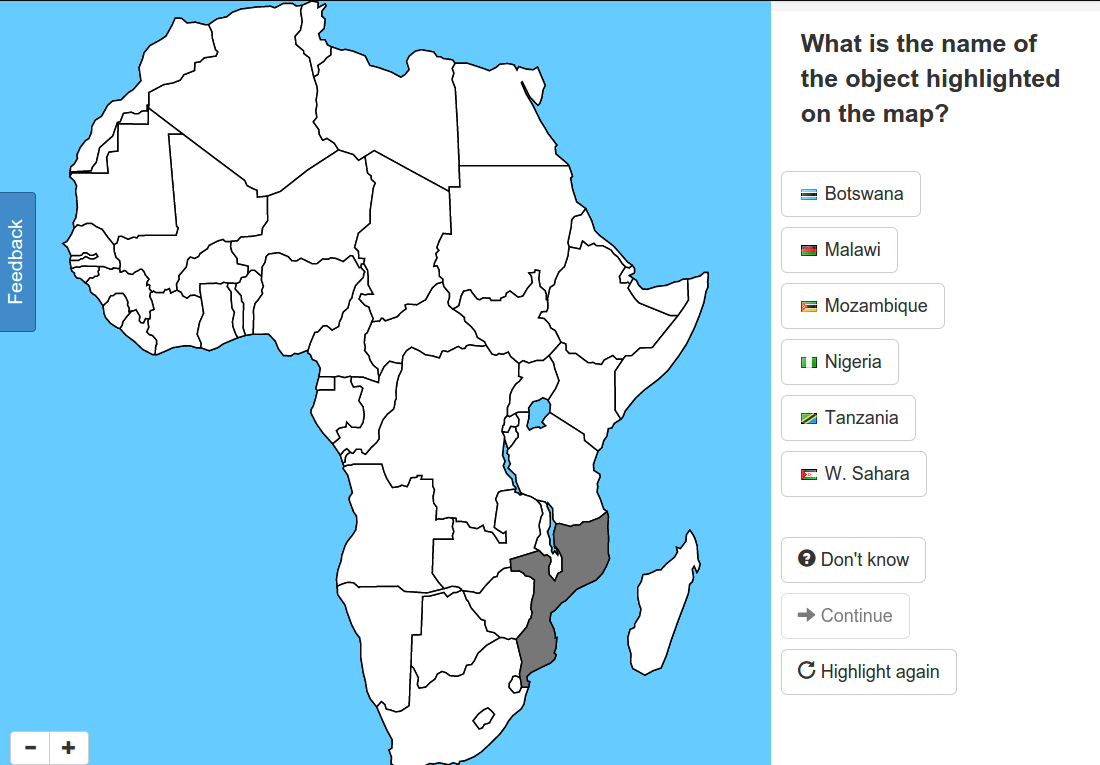
\includegraphics[width=.9\textwidth]{figure/slepemapy_africa_highlighted.png}}
		\only<2>{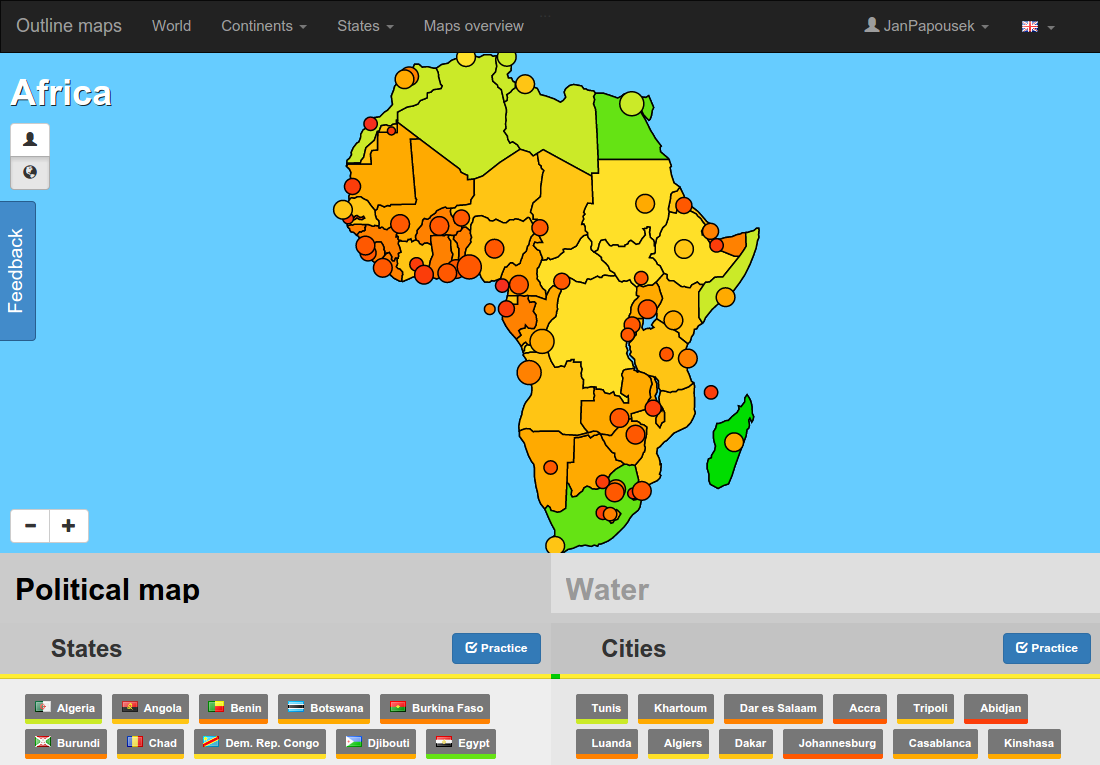
\includegraphics[width=.9\textwidth]{figure/slepemapy_africa.png}}
	\end{center}
\end{frame}
% ------------------------------------------------------------------------------
% --------------------------- SLIDE --------------------------------------------
\begin{frame}
	\frametitle{anatom.cz / practiceanatomy.com}
	\only<1>{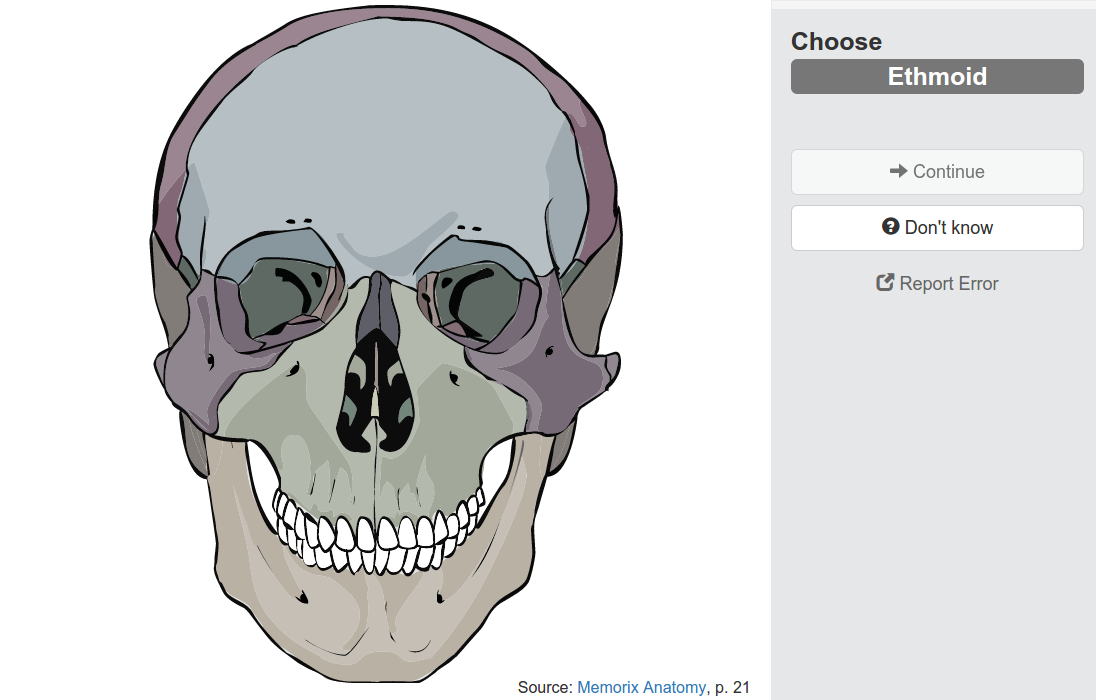
\includegraphics[width=1\textwidth]{figure/anatomy_practice.png}}
	\only<2>{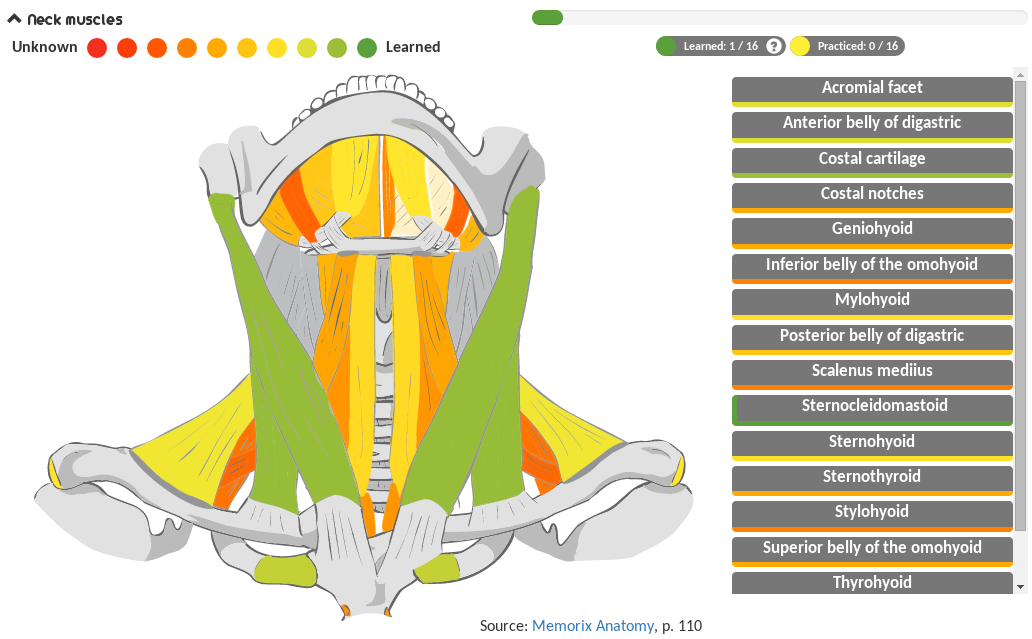
\includegraphics[width=1\textwidth]{figure/anatomy_view.png}}
\end{frame}
% ------------------------------------------------------------------------------
% --------------------------- SLIDE --------------------------------------------
\begin{frame}
	\frametitle{Research Questions}
	\begin{itemize}
		\item \textbf{models}
			\begin{itemize}
				\item How to predict learners' performance based on historical data?
			\end{itemize}
		\item \textbf{practice control}
			\begin{itemize}
				\item How to provide efficient practice with respect to learning and engagement?
			\end{itemize}
		\item \textbf{evaluation}
			\begin{itemize}
				\item How to evaluate proposed approach?
			\end{itemize}
	\end{itemize}
\end{frame}
% ------------------------------------------------------------------------------
% --------------------------- SLIDE --------------------------------------------
\begin{frame}
	\frametitle{State of the Art: Models}
	\textbf{(data) community focuses on procedural knowledge}
	\begin{itemize}
		\item Bayesian Knowledge Tracing and its extensions\\\cite{van2013properties, qiu2011does}
		\item Performance Factor Analysis~\cite{pavlik2009performance}
	\end{itemize}

	\medskip
	\textbf{estimation of prior knowledge can be inspired from testing}
	\begin{itemize}
		\item Item Response Theory~\cite{rasch1993probabilistic,de2008theory}
		\item rating system for chess~\cite{elo1978rating}
	\end{itemize}

	\medskip
	\textbf{learning of factual knowledge}
	\begin{itemize}
		\item forgetting curves~\cite{ebbinghaus1885spacing}
		\item Adaptive Character of Thought-Rational\\\cite{pavlik2005practice}
		\item mixture modeling~\cite{streeter2015mixture}
	\end{itemize}
\end{frame}
% ------------------------------------------------------------------------------
% --------------------------- SLIDE --------------------------------------------
\begin{frame}
	\frametitle{State of the Art: Practice Control}
	\begin{columns}[onlytextwidth]
		\begin{column}{0.4\textwidth}
			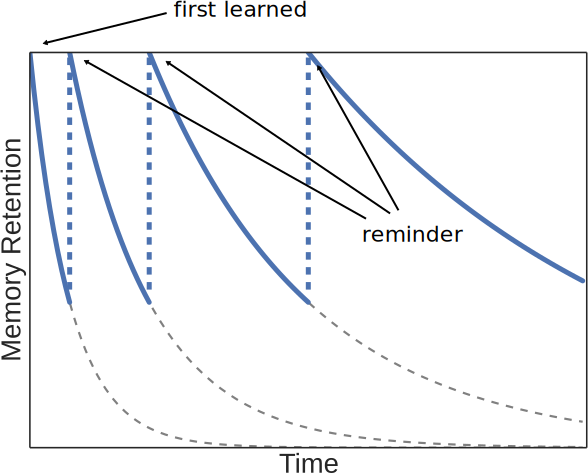
\includegraphics[width=1\textwidth]{figure/forgetting_curves}
		\end{column}
		\begin{column}{0.55\textwidth}
			\begin{itemize}
				\item over-practice vs under-practice\\\cite{cen2007over}
				\item often based on expert's knowledge~\cite{lopes2015multi}
				\item spacing effect~\cite{ebbinghaus1885spacing}
				\item distractors~\cite{little2015optimizing}
			\end{itemize}
		\end{column}
	\end{columns}
\end{frame}
% ------------------------------------------------------------------------------
% --------------------------- SLIDE --------------------------------------------
\begin{frame}
	\frametitle{State of the Art: Evaluation}
	\textbf{historical data}
	\begin{itemize}
		\item performance of predictive models\\\cite{pelanek2014brief, huang2015framework}
	\end{itemize}
	\textbf{new data}
	\begin{itemize}
		\item learning and engagement
		\item offline randomized controlled trials~\cite{dimitrov2003pretest}
		\item online A/B experiments~\cite{stamper2012rise}
		\item multi-armed bandits~\cite{liu2014trading}
	\end{itemize}
	\textbf{synthetic data}
	\begin{itemize}
		\item simulated learners~\cite{fancsali2013optimal}
	\end{itemize}
\end{frame}
% ------------------------------------------------------------------------------
% --------------------------- SLIDE --------------------------------------------
\begin{frame}
	\frametitle{Achieved Results}
	\textbf{slepemapy.cz / outlinemaps.org}
	\begin{itemize}
		\item source of data: almost \numprint{17000000} answers in total
		\item platform for A/B experiments: \numprint{1000000} answers per month
	\end{itemize}
	\textbf{models and practice control}
	\begin{itemize}
		\item combination of Elo rating system and PFA
		\item practice provided with respect to target difficulty\\\cite{papousek2014adaptive}
	\end{itemize}
	\textbf{evaluation}
	\begin{itemize}
		\item impact on engagement~\cite{papousek2015impact}
		\item impact on learning~\cite{papousek2016evaluation}
		\item feedback loop~\cite{niznan2015exploring, pelanek2016impact}
	\end{itemize}
\end{frame}
% ------------------------------------------------------------------------------
% --------------------------- SLIDE --------------------------------------------
\begin{frame}
	\frametitle{Achieved Results: Evaluation}
	\begin{center}
		\only<1>{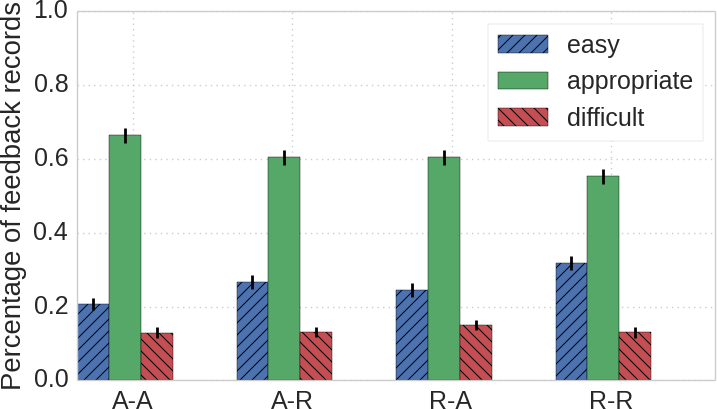
\includegraphics[width=\textwidth]{figure/feedback}}
		\only<2>{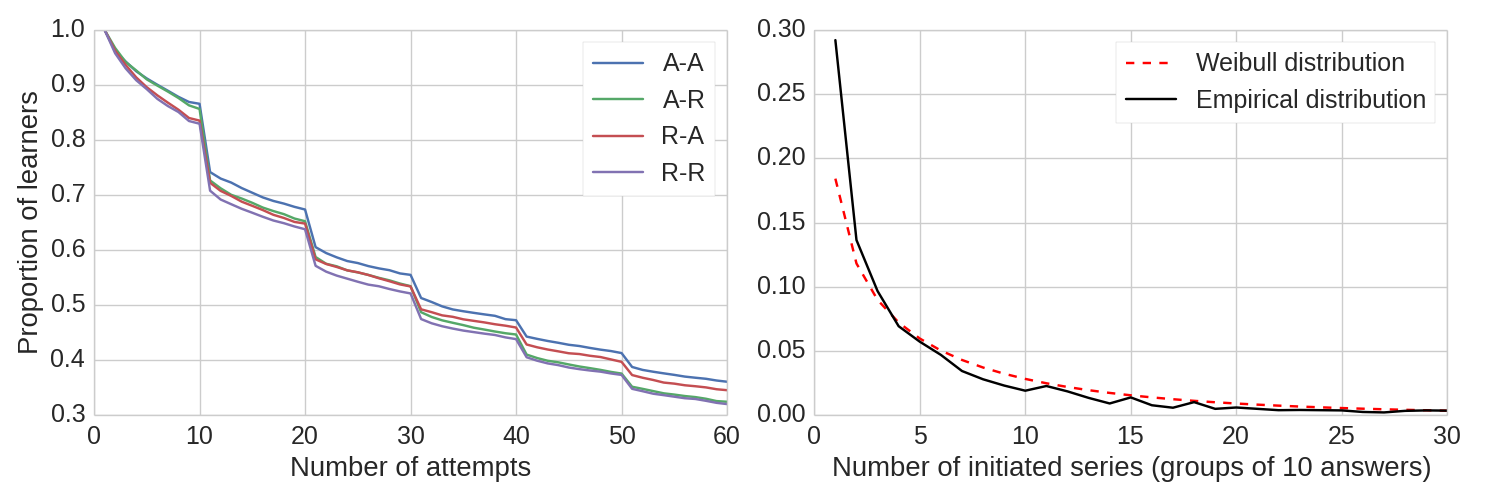
\includegraphics[width=\textwidth]{figure/survivor_curve}}
		\only<3>{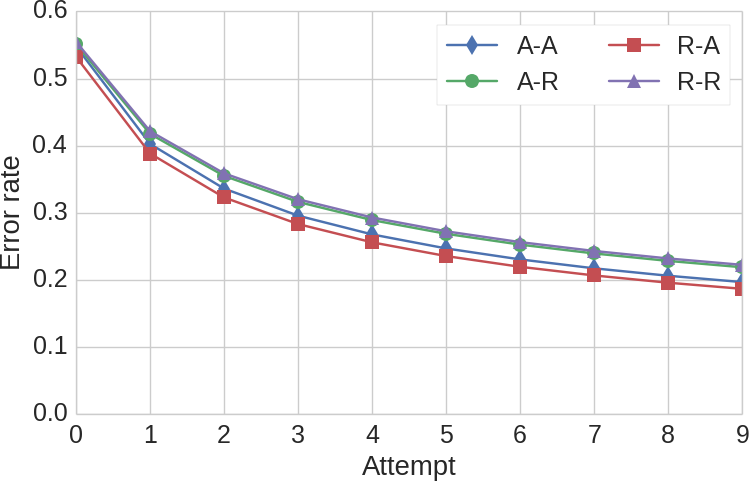
\includegraphics[width=\textwidth]{figure/learning_curve_all_fit}}
	\end{center}
\end{frame}
% ------------------------------------------------------------------------------
% --------------------------- SLIDE --------------------------------------------
\begin{frame}
	\frametitle{Aims of the Thesis}
		\small
		\textbf{models}
		\begin{itemize}
			\item How to efficiently model varied prior knowledge and forgetting?
		\end{itemize}
		\textbf{practice control}
		\begin{itemize}
			\item How to adjust difficulty of practice (spacing vs. number of options)?
			\item Which difficulty is optimal?
			\item How to construct distractors?
		\end{itemize}
		\textbf{evaluation}
		\begin{itemize}
			\item How to measure learning in online environment? (biased data)
			\item What is the effect of feedback loop (model vs. practice control)?
		\end{itemize}
\end{frame}
% ------------------------------------------------------------------------------
% --------------------------- SLIDE --------------------------------------------
\begin{frame}
	\frametitle{Publications}
	\tiny
	{\small \textbf{published}}
	\begin{itemize}
		\item \fullcite{papousek2015impact} (\textbf{best student paper award})
		\item \fullcite{papousek2014adaptive}
		\item \fullcite{papousek2015analysis}
		\item \fullcite{niznan2015exploring}
	\end{itemize}
	{\small \textbf{accepted}}
	\begin{itemize}
		\item \fullcite{papousek2016evaluation}
		\item \fullcite{pelanek2016impact}
		\item \fullcite{papousek2015dataset}
	\end{itemize}
	{\small \textbf{submitted}}
	\begin{itemize}
		\item \fullcite{pelanek2016learner}
	\end{itemize}
\end{frame}
% ------------------------------------------------------------------------------
% --------------------------- SLIDE --------------------------------------------
\begin{frame}
\end{frame}
% ------------------------------------------------------------------------------
% --------------------------- SLIDE --------------------------------------------
\begin{frame}
	\frametitle{Existing tools}
	mainly for vocabulary, e.g.:
	\begin{itemize}
		\item \href{http://duolingo.com}{Duolingo}, \href{http://memrise.com}{Memrise}, \href{http://vocabulary.com}{Vocabulary}
	\end{itemize}
	some general, e.g.
	\begin{itemize}
		\item \href{http://cerego.com}{Cerego}
	\end{itemize}

	\bigskip
	\hrule

	\bigskip
	\begin{itemize}
		\item algorithms often not available
		\item often based on experts' knowledge
	\end{itemize}
\end{frame}
% ------------------------------------------------------------------------------
% --------------------------- SLIDE --------------------------------------------
\begin{frame}
	\frametitle{Model}
	the proposed model should meet the following criteria
	\begin{itemize}
		\item prior knowledge in case of heterogeneous population
		\item learning
		\item forgetting + spacing effect
		\item applicable online
	\end{itemize}
\end{frame}
% ------------------------------------------------------------------------------
% --------------------------- SLIDE --------------------------------------------
\begin{frame}
\frametitle{Proposed Plan of Work}
\begin{tabularx}{\textwidth}{rX}
	\textbf{Autumn 2015} &
		\vspace{-0.5cm}
		\begin{enumerate}
			\item Design and implementation of methodology for evaluation of the impact
				of adaptive practice on a user's learning.
			\item Evaluation of already existing algorithms for practice control using the
				developed methodology.
			\item Deployment of a new version of the system providing the practice of
				geography that will be able to adopt a new student model.
		\end{enumerate}
\end{tabularx}
\end{frame}
% ------------------------------------------------------------------------------
% --------------------------- SLIDE --------------------------------------------
\begin{frame}
\frametitle{Proposed Plan of Work}
\begin{tabularx}{\textwidth}{rX}
	\textbf{Spring 2016} &
		\vspace{-0.5cm}
		\begin{enumerate}
			\item Design and implementation of a new student model of learning of
				facts.
			\item Development of strategies for practice control cooperating with the
				proposed student model.
		\end{enumerate}\\
	\textbf{Autumn 2016} &
		\vspace{-0.5cm}
		\begin{enumerate}
			\item Evaluation of the proposed strategies.
			\item Experiments with synthetic data.
		\end{enumerate}\\
	\textbf{Spring 2017} &
		\vspace{-0.5cm}
		\begin{enumerate}
			\item Finishing and submitting the thesis.
		\end{enumerate}
\end{tabularx}
\end{frame}
% ------------------------------------------------------------------------------
% --------------------------- SLIDE --------------------------------------------
\begin{frame}[t,allowframebreaks]
	\frametitle{References}
	\printbibliography[notcategory=fullcited]
\end{frame}
% --------------------------- SLIDE --------------------------------------------
\end{document}
